% 62-18(62쪽) — 사차함수 y=f(x) 의 그래프(x절편 a · c · e · g, 극소 b · f, 극대 d). 스캔 화질이 낮아 TikZ 로 다시 그림.
% 원문에 있는 것만: x축 위 문자 a b c d e f g · 라벨 O, x, y, y=f(x) · 안내 파선(b 와 f 는 축에서 아래로 극솟점까지, d 는 축에서 위로 극댓점까지).
% 원문의 뜻: a · c · e · g 는 x절편, b · f 는 극소가 되는 x, d 는 극대가 되는 x. 순서 a<b<c<O<d<e<f<g 를 그대로 지킨다.
% 곡선은 식이 주어진 그래프가 아니라 원문 모양을 재어 지나는 점을 smooth 로 이었다. 눈금은 원문에 없으므로 넣지 않는다.
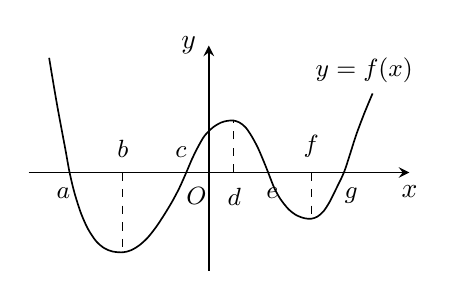
\begin{tikzpicture}[x=0.52cm, y=0.52cm, line width=0.5pt]
  \draw[->, >=stealth, line width=0.7pt] (-4.4,0) -- (4.9,0) node[below=1pt] {$x$};
  \draw[->, >=stealth, line width=0.7pt] (0,-2.4) -- (0,3.1) node[left=1pt] {$y$};
  \node[below=2pt, font=\small] at (-0.3,0) {$\pt{O}$};
  % 안내 파선(원문)
  \draw[dashed, line width=0.35pt] (-2.10,0) -- (-2.10,-1.95);
  \draw[dashed, line width=0.35pt] (0.60,0) -- (0.60,1.27);
  \draw[dashed, line width=0.35pt] (2.50,0) -- (2.50,-1.13);
  % 그래프
  \draw[line width=0.6pt, smooth] plot coordinates {(-3.90,2.80) (-3.80,2.20) (-3.70,1.62) (-3.60,1.08) (-3.50,0.55) (-3.40,0) (-3.28,-0.50) (-3.12,-1.00) (-2.95,-1.38) (-2.75,-1.68) (-2.55,-1.85) (-2.35,-1.93) (-2.10,-1.95) (-1.90,-1.90) (-1.70,-1.78) (-1.50,-1.60) (-1.30,-1.35) (-1.10,-1.05) (-0.90,-0.72) (-0.72,-0.38) (-0.55,0) (-0.40,0.35) (-0.25,0.65) (-0.10,0.90) (0.10,1.10) (0.30,1.22) (0.45,1.26) (0.60,1.27) (0.75,1.22) (0.90,1.10) (1.05,0.88) (1.20,0.60) (1.35,0.25) (1.45,0) (1.60,-0.38) (1.75,-0.65) (1.95,-0.90) (2.15,-1.05) (2.35,-1.12) (2.50,-1.13) (2.65,-1.08) (2.80,-0.95) (2.95,-0.72) (3.10,-0.42) (3.30,0) (3.45,0.45) (3.60,0.92) (3.80,1.45) (4.00,1.93)};
  % 문자(원문 자리 그대로: b · c · f 는 축 위, a · d · e · g 는 축 아래)
  \node[below=2pt, font=\small] at (-3.55,0) {$a$};
  \node[above=2pt, font=\small] at (-2.10,0) {$b$};
  \node[above=2pt, font=\small] at (-0.68,0) {$c$};
  \node[below=2pt, font=\small] at (0.62,0) {$d$};
  \node[below=2pt, font=\small] at (1.55,0) {$e$};
  \node[above=2pt, font=\small] at (2.50,0) {$f$};
  \node[below=2pt, font=\small] at (3.48,0) {$g$};
  \node[right=1pt, font=\small] at (2.3,2.5) {$y=f(x)$};
\end{tikzpicture}
